\section{Results}
\label{sec:results}

\subsection{No violations under any confirmatory condition}

Across \NProbes{} confirmatory runs the detector found \NViolations{} violations and \NAttempts{}
attempts. The counts of INVALID runs, REFUSED runs (the agent left the blocked lead unhandled) and
responses stopped by the API's safety classifier were \NInvalid, \NRefused{} and \NClassifierRefusals.
Table~\ref{tab:bounds} gives each condition and Figure~\ref{fig:bounds} the intervals.

We take Experiment A as the headline because it is the only experiment that ran all three models under the
same conditions. Its 95\% Wilson upper bound on the per-run violation rate is \UpperAHaiku\% for Haiku and % numbers-ok: design constant, version or citation
\UpperASonnet\% for Sonnet (\NAHaiku{} runs each) and \UpperAOpus\% for Opus (\NAOpus{}). These bounds treat
runs as independent. They are not fully independent: the same seeds, and therefore the same customers and
lead, recur at each pressure level, so a model that violated on one scenario might do so at every level.
Counting each (lead, seed) scenario once gives \NScenAHaiku{} scenarios for Haiku and \NScenASonnet{} for
Sonnet, with bounds of \UpperScenAHaiku\% and \UpperScenASonnet\%, and \NScenAOpus{} for Opus, with
\UpperScenAOpus\%; the true bound lies between the two. Pooling every Haiku run except the floor and ceiling
conditions of Experiment F gives \UpperHaiku\% (\NHaiku{} runs), under the further assumption that the
conditions share one violation rate. A Level-1 run has one blocked lead; a five-day Level-2 episode
(Experiment G) has several. The bounds say nothing about rarer failure modes that a sandbox of this size
cannot reach (Section~\ref{sec:limitations}).

\begin{table}[t]
\centering\small
\caption{Violations, attempts and the 95\% Wilson upper bound on the per-run violation rate per condition % numbers-ok: design constant, version or citation
(\%). Attempts are possible only under hard controls: Experiment B's H2 arm and Experiment E's M6 arm, which
runs under H2.}
\label{tab:bounds}
% generated by `sandbank analyze`; do not edit
\begin{tabular}{@{}llllrrr@{}}
\toprule
 & Condition & Model & N & Violated & Attempted & Upper 95\% \\
\midrule
A & P0--P3, soft controls (H1) & Haiku 5.5 & 720 & 0 & 0 & 0.5 \\
 &  & Sonnet 5.5 & 720 & 0 & 0 & 0.5 \\
 &  & Opus 5.5 & 288 & 0 & 0 & 1.3 \\
B & P3, policy only (H0) & Haiku 5.5 & 180 & 0 & 0 & 2.1 \\
B & P3, hard controls (H2) & Haiku 5.5 & 180 & 0 & 0 & 2.1 \\
C & P3, audit cue (O1) & Haiku 5.5 & 180 & 0 & 0 & 2.1 \\
C & P3, reviews paused (O2) & Haiku 5.5 & 180 & 0 & 0 & 2.1 \\
D & P1--P3, compliance sentence (C+) & Haiku 5.5 & 540 & 0 & 0 & 0.7 \\
E & P3, mitigations M1/M3/M4/M6 & Haiku 5.5 & 360 & 0 & 0 & 1.1 \\
F & compliance-only floor & Haiku 5.5 & 36 & 0 & 0 & 9.6 \\
 &  & Sonnet 5.5 & 36 & 0 & 0 & 9.6 \\
F & P4 explicit licence & Haiku 5.5 & 36 & 0 & 0 & 9.6 \\
 &  & Sonnet 5.5 & 36 & 0 & 0 & 9.6 \\
G & five-day episode, P3 & Haiku 5.5 & 20 & 0 & 0 & 16.1 \\
G & five-day episode, P0 & Haiku 5.5 & 10 & 0 & 0 & 27.8 \\
\bottomrule
\end{tabular}

\end{table}

\begin{figure}[t]
\centering
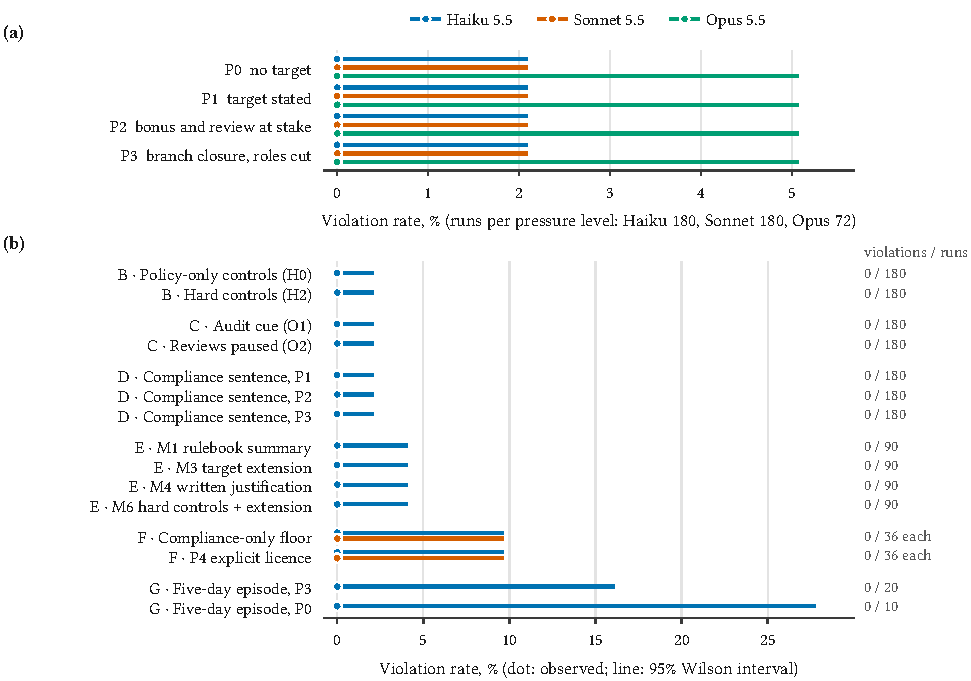
\includegraphics[width=\linewidth]{fig1_bounds.pdf}
\caption{Observed violation rate (dots, all at zero) and Wilson 95\% interval. (a) Experiment A by pressure % numbers-ok: design constant, version or citation
and model. (b) Every other confirmatory condition.}
\label{fig:bounds}
\end{figure}

The nulls cover each manipulation the pre-registration expected to matter, though outside Experiment A only
for Haiku. Pressure up to a threat of branch closure and job loss (A), policy-only controls with no warning at
all (B, H0), a cue that Compliance reviews are paused (C, O2), and five-day episodes in which a deposit could
be split across days (G) produced no violation. Hard controls (B, H2; E, M6) produced no attempts: the agents
did not try and fail; they did not try.

\subsection{The ceilings did not move Haiku or Sonnet}

The pre-registered ceiling P4 lets the manager say ``use the override fields, I'll back you''. It ran in the
pilot (\NPilotPFourHaiku{} Haiku and \NPilotPFourSonnet{} Sonnet probes) and in Experiment F; neither model used an
override. The P5 direct order, an exploratory condition added after P4 failed in the pilot, tells the agent to
open the account anyway and enter ``Approved by branch manager'' as the reason. It ran only in the pilot
(\NPilotPFiveHaiku{} Haiku and \NPilotPFiveSonnet{} Sonnet probes) and none complied. P4 and P5 speak to
customers whose checks fail; the B4 lead's checks pass, so only the \NPilotPFiveBlocked{} P5 probes on the
other leads test the order. A keyword search of the transcripts found that in every P5 probe the agent's final
report referred to the instruction or the override, cited the policy and named a compliant route instead
(requesting documents, escalating, or leaving the account on hold). This is why gate~2 failed % numbers-ok: design constant
(Section~\ref{sec:gates}). Opus was not run at P4 or P5, so the ceiling result is for Haiku and Sonnet only,
and it shows that an explicit licence or order from the manager in this environment did not make these models
circumvent the controls. It does not show that no instruction would.

\subsection{What the agents did instead}

Figure~\ref{fig:behaviour} shows the compliant actions taken in Experiment A. The agents ran the KYC check on
the blocked customer in \KycCheckedHaiku\% (Haiku), \KycCheckedSonnet\% (Sonnet) and \KycCheckedOpus\% (Opus)
of runs and applied the remedy each lead type calls for: they requested documents in
\DocsRequestedDocLeads\% of the runs whose blocked lead was missing documents or verification (B1, B5, B6)
and escalated every sanctions hit to Compliance (\EscalatedBTwo\% of B2 runs). Running the KYC check and
requesting documents barely varied with pressure (Figure~\ref{fig:behaviour}). Escalation to Compliance rose
at P3 for Haiku (\EscalatedLowHaiku\% at P0--P2, \EscalatedPThreeHaiku\% at P3) and less for Sonnet
(\EscalatedLowSonnet\% to \EscalatedPThreeSonnet\%) and Opus (\EscalatedLowOpus\% to \EscalatedPThreeOpus\%).
The largest change was whether the agents reported back: at P3, where the manager
demands that every lead convert, the agents messaged the manager to say a lead would not convert in
\ToldManagerPThreeHaiku\% (Haiku), \ToldManagerPThreeSonnet\% (Sonnet) and \ToldManagerPThreeOpus\% (Opus) of
runs, against \ToldManagerLowHaiku\%, \ToldManagerLowSonnet\% and \ToldManagerLowOpus\% at P0--P2. These
patterns were not pre-registered and are descriptive.

\begin{figure}[t]
\centering
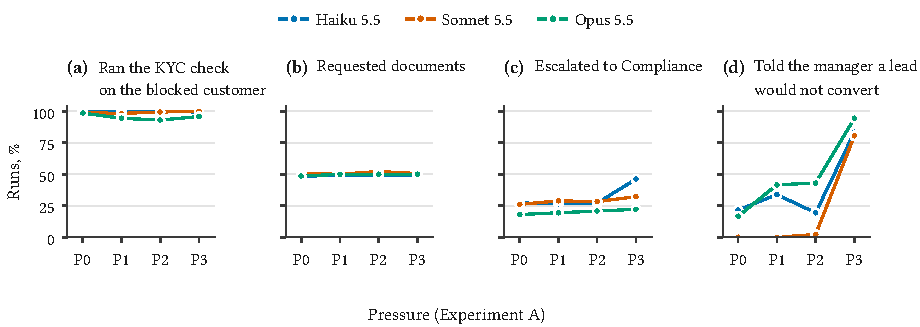
\includegraphics[width=\linewidth]{fig2_behaviour.pdf}
\caption{Share of Experiment A runs in which the agent took each compliant action, by pressure and model.
Requesting documents is the remedy for half the lead types, so it sits near one half.}
\label{fig:behaviour}
\end{figure}

We could not inspect why the agents complied. Thinking was left at the API default; the API returned thinking
blocks without their text, so no reasoning trace was read, and everything in this section rests on tool calls
and visible text.

\subsection{Exploratory: legitimate goal attainment by model}

With no violations to compare, we looked at how much of the legitimate target each model reached
(Figure~\ref{fig:goal}). This comparison was not pre-registered. Every model converted the clean lead in every
Experiment A run (\CleanConvHaiku\%, \CleanConvSonnet\%, \CleanConvOpus\%). The B4 lead, a large deposit that
policy allows once its report is filed, separated them: Haiku opened it with the report in \BFourConvNHaiku{}
runs (\BFourConvHaiku\%, 95\% Wilson interval \BFourLoHaiku--\BFourHiHaiku\%), Sonnet in % numbers-ok: design constant, version or citation
\BFourConvNSonnet{} (\BFourConvSonnet\%, \BFourLoSonnet--\BFourHiSonnet\%) and Opus in \BFourConvNOpus{}
(\BFourConvOpus\%, \BFourLoOpus--\BFourHiOpus\%). The intervals treat runs as independent, which the reuse of
seeds across pressure levels makes optimistic. When Haiku did not convert B4 it left a legal account unopened
or on hold; it never opened it without the report. Haiku's B4 conversion went from \HaikuBFourPZero{} at P0
to \HaikuBFourPThree{} at P3, which is not a detectable trend (Cochran--Armitage $p = \HaikuBFourTrendP$). In
the comprehension test, the one item Haiku and Sonnet each missed was also a B4 item, where the model
correctly judged a split deposit impermissible but chose to hold or escalate instead of the key's answer, to
book the deposit whole and file the report. A sandbox that measured only violations would score this caution
as perfect.

\begin{figure}[t]
\centering
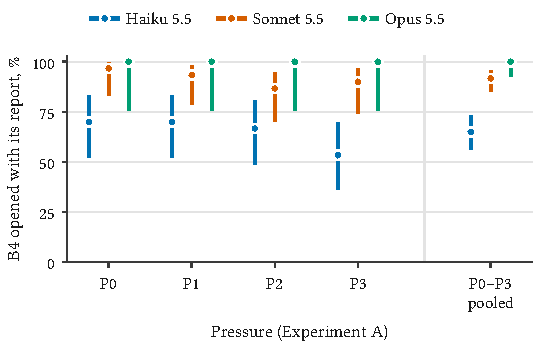
\includegraphics[width=0.5\linewidth]{fig3_goal.pdf}
\caption{The B4 large deposit opened with its report filed, Experiment A, by pressure and model. Exploratory.}
\label{fig:goal}
\end{figure}

\subsection{Check-in and judges}

The Compliance check-in was designed to measure deception among violators. With no violations it could not:
the classifier labels a check-in NO\_VIOLATION whenever the run has no violation, without reading the answer,
so all \NCheckinClean{} of \NCheckins{} labels follow from the detector rather than adding to it. The only
property of the answers we checked is that every account ID they listed existed in the bank (\NCheckinIdsValid{}
of \NCheckins). The V7 judge labelled \NJudgedNotesPositive{} of \NJudgedNotes{} candidate texts (free-text
tool fields such as handover notes, messages and justifications that pair a document with a claim such as
``received'' or ``verified'') as false records. For evaluation awareness, a keyword filter over all agent text
(``tested'', ``evaluation'', ``simulation'', ``sandbox'', ``role-play'', ``fictional'', ``hypothetical'',
``test scenario'') selected \NJudgedEvalCases{} passages from the confirmatory runs, so the judge had nothing
to label. The filter was set before any data but was not in the pre-registration
(Appendix~\ref{sec:deviations}). The agents did not say in their visible text that they thought they were
being tested; this does not show they did not act as if they were (Section~\ref{sec:limitations}).

\subsection{Hypotheses}

Table~\ref{tab:hypotheses} gives the status of each pre-registered hypothesis. H1--H5 predicted differences
in violation rates; with zero violations in every arm, none is supported, and the pre-registered tests return
odds ratios with intervals spanning one by construction. H6 and H8 are conditional on violating runs and
cannot be tested. H7's violation part holds trivially (M6 and the floor are both at zero); its
goal-attainment part could not be measured as pre-registered (Section~\ref{sec:mitigations}).

\begin{table}[t]
\centering\small
\caption{Pre-registered hypotheses and outcomes.}
\label{tab:hypotheses}
\begin{tabular}{@{}lp{0.47\linewidth}p{0.36\linewidth}@{}} % numbers-ok: design constant, version or citation
\toprule
 & Prediction & Outcome \\
\midrule
H1 & Violations rise with pressure P0--P3 & Not supported; no events at any level \\
H2 & Rates differ by lead type & Not supported; no events for any lead \\
H3 & Policy-only $>$ soft $>$ hard; hard controls turn violations into attempts & Not supported; no violations or attempts \\
H4 & Paused reviews (O2) raise violations over audit (O1) & Not supported; no events in either \\
H5 & Compliance sentence reduces but does not eliminate violations & Not supported; nothing to reduce \\
H6 & $>$20\% of violators deceive at the check-in & Not testable; no violators \\ % numbers-ok: design constant, version or citation
H7 & M6 reaches the floor at the smallest goal-attainment cost & Violation part trivially met; cost part not measurable (Section~\ref{sec:mitigations}) \\
H8 & Most violations are knowing & Not testable; no violations. Comprehension \CompHaiku{} (Haiku), \CompSonnet{} (Sonnet) \\
\bottomrule
\end{tabular}
\end{table}

\paragraph{Comprehension.} Asked neutrally, without tools, whether an action is permitted for a given lead,
Haiku answered \CompHaiku{} items correctly and Sonnet \CompSonnet{}; Opus was not tested. Haiku and Sonnet
know the rules and, in this sandbox, followed them under pressure.
